\section{Overall Description}\label{sec:overall-description}
    \subsection{Product Perspective}\label{sec:product-perspective}
        % \emph{Describe the context and origin of the product being specified in this SRS. For example, state whether this product is a follow-on member of a product family, a replacement for certain existing systems, or a new, self-contained product. If the SRS defines a component of a larger system, relate the requirements of the larger system to the functionality of this software and identify interfaces between the two. In this part, make sure to include a simple diagram that shows the major components of the overall system, subsystem interconnections, and external interface. In this section it is crucial that you will be creative and provide as much information as possible.\gnl Provide at least one paragraph describing product perspective. Provide a general diagram that will illustrate how your product interacts with the environment and in what context it is being used, i.e., context diagram.}
        \projectName\ is a standalone product that provides functionality as described in section~\ref{sec:functionality}. It is \gls{open-source} under the \gls{our-license}. The origin of the product comes from desiring automation and streamlined communication within music education. The product itself is made up of two key parts; The frontend provides users an intuitive and functional interface that abstracts away the operations the backend is doing to provide functionality.
        \\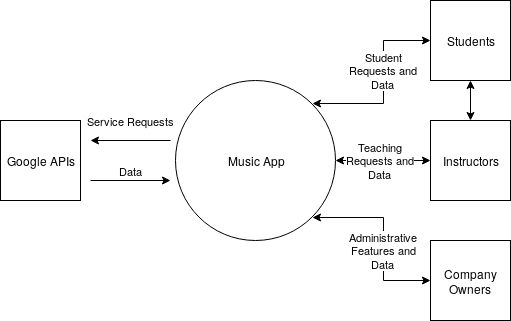
\includegraphics[width=\textwidth]{images/Context-Diagram.png}
        \begin{itemize}
            \item System interfaces
            \item User interfaces
            \item Hardware interfaces
            \item Software interfaces
            \item Communication interfaces
            \item Memory constraints
        \end{itemize}
    \subsection{Product Functionality}\label{sec:product-functionality}
        % \emph{Summarize the major functions the product must perform or must let the user perform. Details will be provided in Section 3, so only a high level summary is needed here. Organize the functions to make them understandable to any reader of the SRS. A picture of the major groups of related requirements and how they relate, such as a top level data flow diagram or object class diagram, will be effective.\begin{enumerate}\item Provide a bulleted list of all the major functions of the system.\item (Optional) Provide a Data Flow Diagram of the system to show how these functions relate to each other. This is useful when there is a clear sequence for the functions being performed.\end{enumerate}}
        \begin{itemize}
            \item Administrative
            \begin{itemize}
                \item \textbf{Add/remove student}. 
                \item \textbf{Add/remove instructor}. 
                \item \textbf{Hierarchy of permissions between user groups}.
            \end{itemize}
            \item File-sharing
            \begin{itemize}                
                \item \textbf{Create and share file templates}.
                \item \textbf{Share files with specific read/write permissions to other users}.
            \end{itemize}
            \item Communications
            \begin{itemize}
                \item \textbf{Ability to message other users}. \emph{As widespread as sending notice to all students of vacation time, or as specific as notifying a certain student of some new material}
                \item \textbf{Default communications to parental units if student is adolescent}.
                \item \textbf{Alerts of varying priority levels}. \emph{Examples include notifying all students of snow day, letting teachers know a student will be on vacation, school requesting an instructor for a certain instrument for a variety of time slots, teachers letting individual students know what to work on or sending additional resources.}
            \end{itemize}
            \item 3rd party integration
            \begin{itemize}                
                \item \textbf{Integration with popular calendars (Apple Calendar, Google Calendar, etc\dots)}. \emph{Instructors could set their available times, schools and students could see such times and request lessons then. Most lessons would be recurring weekly at the same time, optimize for that case.}
            \end{itemize}
            \item \textbf{}.
        \end{itemize}
    \subsection{Users and Characteristics}\label{sec:users-characteristics}
        % \emph{Identify the various users that you anticipate will use this product. Users may be differentiated based on frequency of use, subset of product functions used, technical expertise, security or privilege levels, educational level, or experience.\begin{enumerate}\item Describe the pertinent characteristics of each user. Certain requirements may pertain only to certain users.\item Distinguish the most important users for this product from those who are less important to satisfy.\end{enumerate}}
        There are 3 main groups of users for \projectName:
        \begin{enumerate}
            \item \textbf{Music schools}. Music schools manage the instructors and students under their umbrella of operation. They have permissions to add/remove association with the other user types, as well as special operations regarding interactions between the user groups.
            \item \textbf{Music instructors}. Instructors interact with their associated companies and students. The students can be private or managed by a music school. Instructors are primarily responsible for \glspl{lesson plan} and \glspl{practice-resource} for their students, and sharing such resources with schools or other teachers. Instructors are the primary intended client as they have the most to benefit from the product's functionalities.
            \item \textbf{Music students}. Students have access to a history of their \glspl{lesson plan}, \glspl{practice-resource}, and communication with their associated instructor or school. 
            % \item \textbf{Administrator of student account}. Possible administrators of student accounts would be parents/guardians of a young student. The parent can monitor their child's interactions and manage permissions \emph{(such as allowing the student to read messages but not send replies, or get notifications when the student does some activity)}.
        \end{enumerate}
    \subsection{Operating Environment}\label{sec:operating-environment}
        % \emph{Describe the environment in which the software will operate, including the hardware platform, operating system and versions, and any other software components or applications with which it must peacefully coexist. In this part, make sure to include a simple diagram that shows the major components of the overall system, subsystem interconnections, and external interface.\gnl As stated above, in at least one paragraph, describe the environment your system will have to operate in. Make sure to include the minimum platform requirements for your system.}
        \projectName\ will run in a \gls{kubernetes} cluster hosted on a cloud platform such as \gls{aws} or \gls{gcp}. The programs themselves will run as \gls{docker} containers. The compute nodes will need to be able to run several micro services and visibility plugin applications.
    \subsection{Design and Implementation Constraints}\label{sec:design-constraints}
        \emph{Describe any items or issues that will limit the options available to the developers. These might include: hardware limitations (timing requirements, memory requirements); interfaces to other applications; specific technologies, tools, and databases to be used; parallel operations; language requirements; communications protocols; security considerations; design conventions or programming standards (for example, if the customer’s organization will be responsible for maintaining the delivered software).\gnl In this section you need to consider all of the information you gathered so far, analyze it and correctly identify relevant constraints.}
        \subsubsection{Language Requirements}
            The backend will be written primarily in \gls{go}. The frontend will utilize \acrshort{html}, \acrshort{css}, and \acrfull{ts}.
        \subsubsection{Technology Stack}
            \begin{itemize}
                \item \gls{vue}
                \item \gls{gcp}
                \item \gls{kubernetes}
                \item \gls{docker}
                \item GitHub
            \end{itemize}
        \subsubsection{External Interfaces}
            \begin{itemize}
                \item Google Calendar
                % \item Jackrabbit Music
            \end{itemize}
        \subsubsection{Development Environment}
            \todo Mention cross-platform development compatibility, and being able to run the full stack locally with \gls{docker} for testing purposes.
    \subsection{User Documentation}\label{sec:user-documentation}
        % \emph{List the user documentation components (such as user manuals, on-line help, and tutorials) that will be delivered along with the software. Identify any known user documentation delivery formats or standards.\gnl You will not actually develop any user-manuals, but you need to describe what kind of manuals and what kind of help is needed for the software you will be developing. One paragraph should be sufficient for this section.}
        Along with the product, basic user manuals and guides will be provided. Text tutorials for common workflows and functionalities will be found on the site. To aid in creating a better user experience, there should also be a way for users to request new documentation or submit issue reports.
    \subsection{Assumptions and Dependencies}\label{sec:assumptions-dependencies}
        \emph{List any assumed factors (as opposed to known facts) that could affect the requirements stated in the SRS. These could include third-party or commercial components that you plan to use, issues around the development or operating environment, or constraints. The project could be affected if these assumptions are incorrect, are not shared, or change. Also identify any dependencies the project has on external factors, such as software components that you intend to reuse from another project.\gnl Provide a short list of some major assumptions that might significantly affect your design. For example, you can assume that your client will have 1, 2 or at most 50 Automated Banking Machines. Every number has a significant effect on the design of your system.}
